\subsection{Hypothesis on Relation Properties}
\label{sec:hypothesis_relation_properties}

This hypothesis is inspired by the fact that some embedding methods are unable to handle specific properties.

%\begin{figure*}[htb]
\centering
\begin{minipage}{0.95\textwidth}
\centering
\small
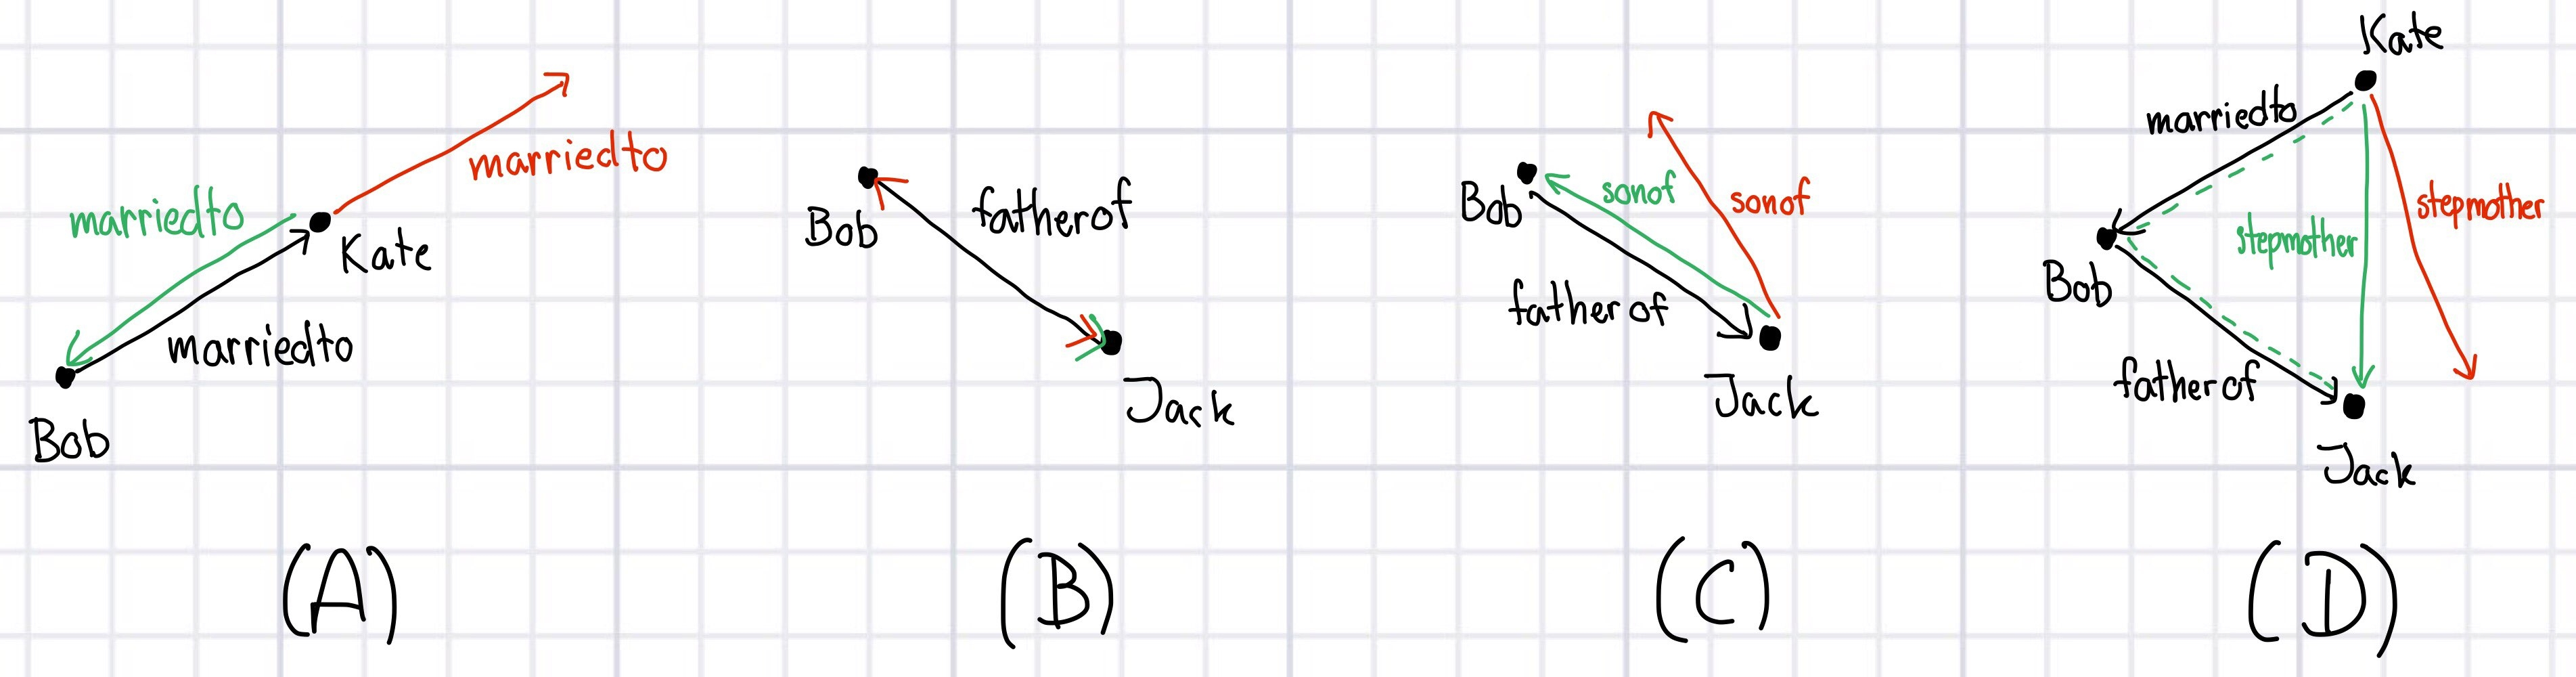
\includegraphics[scale=0.12]{content/hypotheses/figures/relation_properties_A-D.jpg}
\caption{Illustration of \autoref{hyp:relation_properties} A-D. Black is embedded information and red/green are different versions of the same relation embedding. Green is what the embedding should look like if the method can model relations with that property and red is what the embedding might look like if not. A: Symmetry, B: Anti-Symmtery, C: Inversion, D: Composition.
}
\label{fig:relation_properties_nothierarchy}
\end{minipage}
\end{figure*}
%\begin{figure*}[htb]
\centering
\resizebox{\textwidth}{!}{
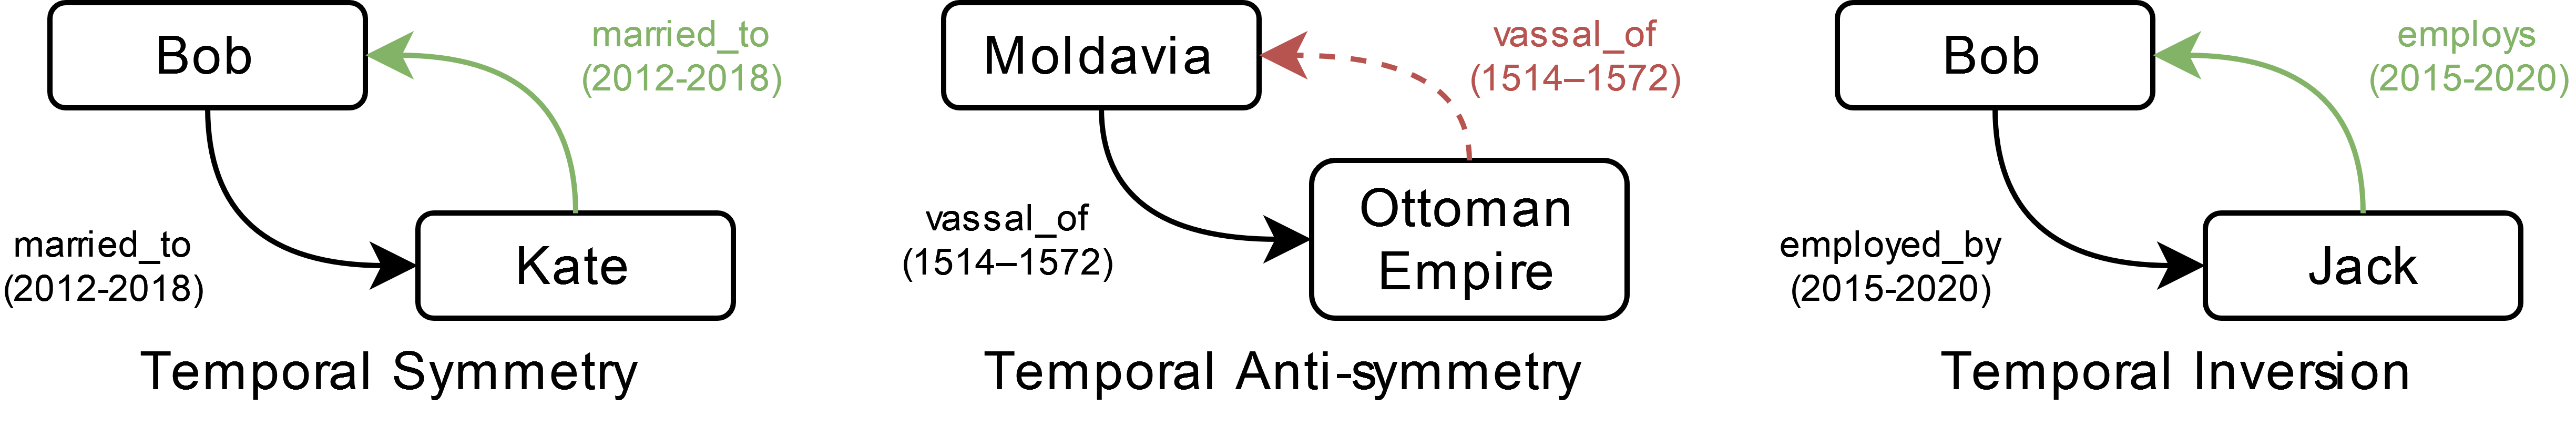
\includegraphics{content/hypotheses/figures/relation_properties.png}
}
\centering
\begin{minipage}{\fullwidthcaption}
\caption{Examples of temporal relation properties. Green relations mean that the relation must exist for the relation to have the given property. Red means that the relation must not exist for the relation to have that property.}
\label{fig:relation_properties_nothierarchy}
\end{minipage}
\end{figure*}

\begin{hypothesis}
\label{hyp:relation_properties}
Prediction quality of queries with certain temporally constrained relation properties is significantly higher on methods, which theoretically can model those properties, than methods which cannot.
\end{hypothesis}

For this hypothesis we compare DE-TransE, DE-DistMult and DE-SimplE as they resemble one another and have varied combinations of relation properties that they can and cannot model.
For more information on the selected methods see \autoref{sec:methods}.

The relation properties selected for analysis are symmetry, antisymmetry, and inversion. Reflection, composition and hierarchy were considered but disregarded. 
Reflection was disregarded because all considered methods are capable of modeling it and because we found no relation with that property in any of the datasets.
Composition was disregarded because composition is made up of multiple facts, and as such it is more affected by incomplete data than other relation properties. Additionally, we found no occurences of composition in the data, possibly due to aforementioned vulnerability.
Hierarchy was disregarded as we were unable to identify a \gls{kge} method which was both capable of modeling that relation property and temporal.

This hypothesis is divided into several subhypotheses specific to each relation property.

\begin{subhypothesis}
\label{hyp:relation_property_sym}
DE-TransE has worse performance than DE-DistMult and DE-SimplE on link prediction tasks in which the relation in the queries has the \textbf{symmetric} property.
\end{subhypothesis}

As TransE is a straightforward translational method in Euclidian space, it is incapable of modelling symmetry \cite{goel19diachronicemb}. Theoretically, DE-TransE has the same limitation with temporal symmetric relations, which are relations that happen simultaniously between two entities. 
An example of such a relation could be \textit{is\_married}. The problem is illustrated in \autoref{fig:detranse_is_married}. 
The purpose of \autoref{hyp:relation_property_sym} is to empirically analyze the practical impact of this theoretical limitation.

\newcommand{\ismarried}[0]{
    node [
            near start, 
            above=5pt,
            color=black!80,
            align=center,
            execute at begin node=\setlength{\baselineskip}{4pt},
        ] 
        {is married\\\footnotesize{2018-2023}}
}

\begin{figure}[htb]
\centering

\begin{tikzpicture}
    \node [draw, circle, outer sep=2pt] (John) at (0,0){John};
    \node [draw, circle, outer sep=2pt] (Jane) at (3,1){Jane};
    \node [draw, circle, densely dotted, scale=3, outer sep=2/3pt] (unknown) at (6,2){};
    \draw [ultra thick, ourdarkgreen, ->] (John) -- (Jane) \ismarried ;
    \draw [ultra thick, ourdarkyellow, ->] (Jane) -- (unknown) \ismarried ;
\end{tikzpicture}
\centering

\begin{minipage}{\columnwidthcaption}
\caption{Illustration of DE-TransE embedding of the relation \textit{is\_married}. John is married to Jane, which is modelled with a translation from John to Jane (green), but when the same translation is applied to Jane the result is unknown (yellow).}
\label{fig:detranse_is_married}
\end{minipage}

\end{figure}

\begin{subhypothesis}
\label{hyp:relation_property_antisym}
DE-DistMult has worse performance than DE-TransE and DE-SimplE on link prediction tasks in which the relation in the queries has the \textbf{antisymmetric} property.
\end{subhypothesis}

DistMult uses pairwise interactions in diagonal matrices, and as such cannot model edge direction, which in turn means it cannot model antisymmetry \cite{goel19diachronicemb}. Theoretically, DE-DistMult has the same problem, but for temporal antisymmetric relations, which are relations where an entity performs an action to another entity and that other entity cannot do the same action back in the same timespan. 
An example of such a relation is \textit{owes money}, as two people cannot owe eachother money as one debt will cancel out the other.
The problem is illustrated in \autoref{fig:dedistmult_owes_money}.
The purpose of \autoref{hyp:relation_property_antisym} is to empirically analyze the practical impact of this theoretical limitation.

\newcommand{\cellsize}{0.9cm}
\newcommand{\owesmoney}{\textit{owes}\\\textit{money}}
%\newcommand{\hatch}{[pattern=north east lines, pattern color=ourdarkblue]}

\begin{figure}[htb]
\centering
\begin{tikzpicture}
    \tikzstyle{hatch}=[
        pattern=north west lines,
        pattern color=ourgrey,
        ]
    \tikzstyle{every node}=[
        inner sep=0pt,
        %draw=black,
        x=\cellsize, 
        y=\cellsize,
        minimum size=\cellsize,
        align=center,
        execute at begin node=\setlength{\baselineskip}{6pt},
        font=\small,
        ]
    \pgfmatrix{rectangle}{center}{mymatrix}
    {\pgfusepath{}}{\pgfpointorigin}{\let\&=\pgfmatrixnextcell}
    {
        \node(0_0) {\owesmoney};    \& \node(1_0){Jack}; \& \node(2_0) {Peter}; \& \node(3_0) {Kate};\\
        \node(0_1) {Jack};               \& \node(1_1){}; \& \node(2_1) {\scaleto{\textbf{$\times$}}{10pt}}; \& \node(3_1){};\\
        \node(0_2) {Peter};              \& \node(1_2)[hatch] {}; \& \node(2_2) {}; \& \node(3_2){};\\
        \node(0_3){Kate};                \& \node(1_3)[hatch] {}; \& \node(2_3)[hatch]{}; \& \node(3_3){};\\
    }
    \draw (0_0.south west) -- (3_0.south east) (0_1.south west) -- (3_1.south east) (0_2.south west) -- (0_2.south east) (2_2.south west) -- (3_2.south east);
    \draw (0_0.north east) -- (0_3.south east) (1_0.north east) -- (1_2.south east) (2_0.north east) -- (2_3.south east) ;
\end{tikzpicture}
\centering

\begin{minipage}{\columnwidthcaption}
\caption{Illustration of DE-DistMult embedding of the relation \textit{owes money}. The relation exists between Jack and Peter, but it is unknown who owes who money. DistMult cannot model the hatched cells.}
\label{fig:dedistmult_owes_money}
\end{minipage}

\end{figure}

%\def\mystrut(#1,#2){\vrule height #1 depth #2 width 0pt}
% \newcolumntype{C}{%
%    >{\mystrut(3ex,3ex)\centering}%
%    p{3ex}%
%    <{}}  

% \begin{tabular}{r|C|c|c}
% %|*{6}{p{1.5cm}|}}
% \textit{Arrest} & Jack & Peter & Louise\\
% \hline
% Jack    & False             & True              & False \\
% \hline
% Peter   & \cellcolor{gray}  & False             & False \\
% \hline
% Louise  & \cellcolor{gray}  & \cellcolor{gray}  & False \\
% \end{tabular}

\begin{subhypothesis}
\label{hyp:relation_property_inv}
DE-DistMult has worse performance than DE-TransE and DE-SimplE on link prediction tasks in which the relation in the queries has the \textbf{inversion} property.
\end{subhypothesis}

As DistMult cannot model edge direction, it also cannot model inversion \cite{goel19diachronicemb}. Theoretically, DE-DistMult has the same problem, but for temporal inverse relations, which are pairs of relations, where when one entity relates to another with one type, they are also related in the opposite direction with the other type, both relations happening in the same timespan. An example of such a pair is the relations \textit{host\_a\_visit} and \textit{make\_a\_visit}. The purpose of \autoref{hyp:relation_property_inv} is to empirically analyze the practical impact of this theoretical limitation.

To analyze these subhypotheses, the test sets are divided into sets of facts that contain only relations of that type and sets of facts that contain all but that relation. The first step is to assign a number of soft labels to each relation, using a function for each relation property that maps each relation to a real number $\varR \rightarrow [ 0 , 1 ]$. 
We define a threshold for each of the relation properties, and classify each relation as being symmetric, antisymmetric, and/or inverse if the soft label for that relation is higher than or equal to the threshold.
Alternative approaches are discussed in \autoref{sec:alt_approaches_to_relation_properties}. This function describes how many facts fulfill the requirements for that relation. The reason soft labels are used is that \glspl{tkg} are not complete, and some relations might be missing from the graphs.

The symmetry soft label for relation $r$ is

\begin{equation}
\begin{gathered}
\mathit{sym}(r) = \frac{|S|}{|\eta_r|}\\
S = \{ (e_1, r, e_2, \tau) \in \eta_r \mid (e_2, r, e_1, \tau) \in \eta_r \}
\end{gathered}
\end{equation}

\noindent
where $\eta_r \subset \varG$ is the set of all facts in $\varG$ where the relation is $r$, $e_1, e_2 \in \varE$, and $\tau$ is a timespan. 

The antisymmetry soft label for relation $r$ is

\begin{equation}
\begin{gathered}
\mathit{asym}(r) = \frac{|A|}{|\eta_r|}\\
A = \{ (e_1, r, e_2, \tau) \in \eta_r \mid (e_2, r, e_1, \tau) \notin \eta_r \}
\end{gathered}
\end{equation}

The inversion soft label for relation $r$ is

\begin{equation}
\begin{gathered}
\mathit{inv}(r) = \varmax_{r^n \in \varR \setminus \{r\} } \frac{|I_{r^n}|}{|\eta_{r^n}|}\\
I_{r^n} = \{ (e_2, r^n, e_1, \tau) \in \eta_{r^n}  \mid (e_1, r, e_2, \tau) \in \eta_r \}
\end{gathered}
\end{equation}

\noindent
where $\varR \setminus \{r\}$ is $\varR$ without the element $r$.
$\mathit{inv}(r)$ finds the $r^n$ with the highest percentage of instances where there for a fact $(e_1, r, e_2, \tau)$ exists a different fact $(e_2, r^n, e_1, \tau)$.

% \noindent
% The reflexivity soft label for relation $r$ is

% \begin{equation}
% \begin{gathered}
% \mathit{ref}(r) = \frac{|R|}{|\eta_r|}\\
% R = \{ (e_1, r, e_2, \tau) \in \eta_r \mid e_1 = e_2 \}
% \end{gathered}
% \end{equation}

Any relation can be classified with any number of relation properties. The threshold for symmetry is $0.8$, for antisymmetry is $1.0$, and for inverse is $0.8$.
The set of facts where the relation is symmetric ($T_S$), as well as the set of test facts where the relation is non-symmetric ($T_S'$), on test set $T$ is defined

\begin{equation}
\begin{aligned}
T_S & = \{ f \in T \mid \mathit{sym}(r) \geq 0.8 \}\\
T_S' & = \{ f \in T \mid \mathit{sym}(r) < 0.8 \}
\end{aligned}
\end{equation}

\noindent
Similarly, the antisymmetric test facts $T_A$, the non-antisymmetric test facts $T_A'$, the inverse test facts $T_I$, and the non-inverse test facts $T_I'$ are defined, using their respective thresholds.

The models are evaluated over these property specific test sets for each dataset and compared to one another. 
The difference between the score of the test set of a relation property and the test set without that relation property is worse for a model that cannot express that relation property than the difference between those scores for models that can express that property.
If this is the case the hypothesis is deemed true.